\documentclass[11pt,reqno]{amsart}

\usepackage[margin=1.05in]{geometry}
\usepackage{amsmath,amssymb,amsthm,mathtools}
\usepackage{booktabs,array}
\usepackage{graphicx}
\usepackage{xcolor}
\usepackage{hyperref}

\definecolor{navy}{HTML}{0F172A}
\definecolor{accent}{HTML}{1D4ED8}
\hypersetup{
  colorlinks=true,
  linkcolor=accent,
  citecolor=accent,
  urlcolor=accent,
  pdftitle={Minimax Recovery of Polygon Corner Charges from Bandlimited Leont'ev Frequencies: Parity, Angle-Dependent Exponents, and Super-Resolution}
}

\newtheorem{theorem}{Theorem}[section]
\newtheorem{proposition}[theorem]{Proposition}
\newtheorem{lemma}[theorem]{Lemma}
\newtheorem{corollary}[theorem]{Corollary}
\theoremstyle{definition}
\newtheorem{definition}[theorem]{Definition}
\newtheorem{openproblem}[theorem]{Open Problem}
\theoremstyle{remark}
\newtheorem{remark}[theorem]{Remark}

\newcommand{\C}{\mathbb{C}}
\newcommand{\R}{\mathbb{R}}
\newcommand{\Z}{\mathbb{Z}}
\newcommand{\N}{\mathbb{N}}
\DeclareMathOperator{\Log}{Log}
\DeclareMathOperator{\dist}{dist}
\DeclareMathOperator{\fp}{fp}

\title[Minimax Recovery of Polygon Corner Charges]{Minimax Recovery of Polygon Corner Charges\\
from Bandlimited Leont'ev Frequencies:\\
Parity, Angle-Dependent Exponents, and Super-Resolution}

\author{Project ReMath}
\date{November 23, 2026}
\subjclass[2020]{Primary 41A46, 65R32; Secondary 30B50, 42A15, 35J05}
\keywords{Optimal recovery, minimax risk, convex polygons, Leont'ev exponential frequencies, boundary Christoffel function, super-resolution, interval arithmetic, Hadamard finite part}

\begin{document}

\begin{abstract}
On a bounded convex $p$-gon $D \subset \C$ with counterclockwise vertices $\gamma_1,\dots,\gamma_p$ and edge vectors $d_j = \gamma_{j+1}-\gamma_j$, A.~F.~Leont'ev's canonical exponential lattice $\Lambda_+ = \{\nu_{jm} = 2\pi i m / d_j : 1 \le j \le p,\; m \ge 1\}$ furnishes the natural spectral grid associated with $\partial D$. We study the inverse problem of recovering unknown real point charges $a = (a_1,\dots,a_p) \in \R^p$ at the vertices of $D$ from finitely many bandlimited boundary-transform samples $B_\mu(s) = \int_{\partial D} e^{sw}\,d\mu(w)$ of a composite boundary load $\mu = \sum_{j=1}^p a_j \delta_{\gamma_j} + g\,d\ell$ contaminated by an unknown diffuse flux $g$.

First, we prove that for \emph{any} finite signed background (including singular continuous measures), normalized Ces\`aro averages along edge $j$ converge to $a_j + a_{j+1}$, yielding a sharp polygon parity dichotomy: odd polygons ($p = 2\kappa+1$) identify every vertex charge, whereas even polygons ($p = 2\kappa$) annihilate the alternating mode $(-1)^j$ in the asymptotic endpoint-sum limit, which is unmasked by a fractional shift $m \mapsto m + \theta$ ($\theta \notin \Z$) on a single edge. Second, over the $L^2$ background ball $\|g\|_{L^2(\partial D)} \le M$, we establish the exact finite-band minimax risk over \emph{all linear and nonlinear estimators} via opposite zero-data witnesses. Third, on every odd convex $p$-gon with $N$ integer modes per side, we prove the sharp asymptotic minimax law $E_k = M N^{-1/2}(C_k + o(1))$ ($1 \le k \le p$) with an explicit Hilbert-projection constant $C_k = \|\Pi T^* c^{(k)}\| > 0$ computable via dyadic logarithmic Gram matrices, and prove for $M > 0$ that calibrated Ces\`aro averaging is strictly suboptimal ($\lim_{N\to\infty} E_{k,\mathrm{Ces}}/E_k > 1$). Fourth, on an even convex $p$-gon, appending $N$ shifted samples on a single edge breaks the $N^{-1/2}$ barrier and improves the minimax exponent at vertex $\gamma_k$ to an \emph{angle-dependent} power law $E_k \asymp_D M N^{-(1 - \omega_k/(2\pi))}$ governed by the interior angle $\omega_k$ via Varga's boundary Christoffel estimates---verified across 28 finite-band risks to 45 significant digits on a $60^\circ/120^\circ$ rhombus exhibiting simultaneous $N^{-5/6}$ and $N^{-2/3}$ rates---whereas adding a single shifted frequency yields $\Theta(M)$ floors at fixed or top-of-band placement vs.\ $\Theta(M N^{-1/2})$ in the proportional band interior. Outward-rounded interval certificates on the unit square prove that the intuitive half-step $\theta = 1/2$ is globally suboptimal over $\theta \in (0,1)$ at $N = 1, 2, 4$. Fifth, for edgewise $C^r$, $H^r$, or uniformly analytic backgrounds, identifying inverse-power-annihilating windows achieve $O(N^{-r-1})$, $O(N^{-r-1/2})$, and exponential super-resolution ($1.9\times 10^{-2} \to 6.0\times 10^{-26}$ on the triangle at $N=128$) subject to a universal Chebyshev norm barrier. Finally, we prove an exact Hadamard finite-part identity against entire holomorphic tests reading discontinuous wall-temperature jumps of harmonic plates directly from spectral space. Core algebraic and minimax modules are formally machine-checked in Lean~4.
\end{abstract}

\maketitle

\section{Introduction}

Suppose an unknown boundary distribution $\mu = \sum_{j=1}^p a_j \delta_{\gamma_j} + g\,d\ell$ on the boundary of a bounded convex $p$-gon $D \subset \C$ ($p \ge 3$, genuine counterclockwise vertices $\gamma_1,\dots,\gamma_p$, interior angles $0 < \omega_k < \pi$, edge vectors $d_j = \gamma_{j+1}-\gamma_j$) is probed through its complex exponential transform
\begin{equation}\label{eq:B-transform}
  B_\mu(s) = \int_{\partial D} e^{sw}\,d\mu(w) = \sum_{\ell=1}^p a_\ell e^{s\gamma_\ell} + \int_{\partial D} e^{sw} g(w)\,d\ell(w),
\end{equation}
sampled on finite bands of A.~F.~Leont'ev's canonical polygon lattice \cite{Leontev1974Polygon,Leontev1976Book,Leontev1987TrMIAN}
\begin{equation}\label{eq:lattice}
  \Lambda_+ = \left\{ \nu_{jm} = m b_j : 1 \le j \le p,\; m \in \Z_{\ge 1} \right\},
  \qquad b_j = \frac{2\pi i}{d_j}, \quad c_j = \frac{1}{b_j}.
\end{equation}
Such measurements arise naturally in complex harmonic analysis and in spectral boundary-value solvers (most notably Fokas's Unified Transform Method \cite{FFX2004,Ashton2012,AshtonFokas2013}; see the companion paper \cite{Paper1} for the classification of infinite-band invisible loads on $\Lambda_+$). In physical and PDE settings, point masses $a_j \delta_{\gamma_j}$ model concentrated corner sources or tangential-derivative Dirac jumps $a_j = T_j - T_{j-1}$ caused by discontinuous Dirichlet boundary data at polygon vertices, while $g$ represents an unknown diffuse boundary flux. (Throughout the text we index vertices $1 \le k \le p$; numerical figures use zero-based labels $v_0,\dots,v_{p-1}$ corresponding to $\gamma_1,\dots,\gamma_p$, so $E_0$ denotes $E_1$.)

This paper resolves the quantitative finite-band optimal recovery problem \cite{MicchelliRivlin1977,Donoho1994,DFPW2019}: given $N$ frequency samples per side, how accurately can $a = (a_1,\dots,a_p) \in \R^p$ be reconstructed against worst-case diffuse backgrounds $g$, and can nonlinear estimators or tailored spectral designs outperform classical averaging? Our investigation uncovers five distinct phenomena:
\begin{enumerate}
  \item \emph{Universal endpoint-pair limit and parity dichotomy (Section~\ref{sec:parity})}: Along edge $j$, normalized averages $N^{-1}\sum_{m=1}^N e^{-\nu_{jm}\gamma_j}B_\mu(\nu_{jm})$ converge to $a_j + a_{j+1}$ in the presence of \emph{arbitrary} diffuse or singular continuous measures. Odd polygons ($p = 2\kappa+1$) invert $(a_j + a_{j+1})_{j=1}^p$ uniquely; even polygons ($p = 2\kappa$) lose the alternating vector $(-1)^j$ in the limit, which is restored by shifting $m \mapsto m + \theta$ ($\theta \notin \Z$) on one edge.
  \item \emph{Exact finite-band minimax formula over all nonlinear estimators (Section~\ref{sec:minimax})}: Over the $L^2$ ball $\|g\|_{L^2(\partial D)} \le M$, the minimax risk for coordinate $a_k$ ($1 \le k \le p$) equals $E_k = M\sqrt{K_{kk}}$ in closed form, where $K = (A^T G^{-1} A)^{-1}$ is built from elementary edge exponential integrals, and no nonlinear estimator improves upon the linear saddle-point estimator.
  \item \emph{Sharp odd-polygon $N^{-1/2}$ constant and strict suboptimality of Ces\`aro (Section~\ref{sec:odd})}: On every odd $p$-gon ($M > 0$), $E_k = M N^{-1/2}(C_k + o(1))$ with $C_k = \|\Pi T^* c^{(k)}\| > 0$ characterized by a tangent-ray Hilbert operator and bounded from above by dyadic logarithmic Gram matrices; calibrated Ces\`aro averaging suffers a strict asymptotic penalty $\|T^* c^{(k)}\| / \|\Pi T^* c^{(k)}\| > 1$.
  \item \emph{Angle-dependent exponent jump and failure of half-step optimality on even polygons (Section~\ref{sec:even})}: Appending $N$ shifted samples on a single edge of an even $p$-gon breaks the $N^{-1/2}$ barrier, accelerating the minimax rate at $\gamma_k$ to $E_k \asymp_D M N^{-(1 - \omega_k/(2\pi))}$ via Varga's boundary Christoffel estimates \cite{Varga2013}. Adding only \emph{one} shifted sample exhibits a placement transition ($\Theta(M)$ floor at a fixed node or at $m = N-1$, vs.\ $\Theta(M N^{-1/2})$ in the proportional band interior). Moreover, rigorous interval arithmetic certifies that the intuitive half-step $\theta = 1/2$ is globally suboptimal on the unit square at $N = 1, 2, 4$.
  \item \emph{Smooth-background super-resolution, Chebyshev barrier, and discontinuous heated plates (Sections~\ref{sec:superres}--\ref{sec:plates})}: Annihilating the asymptotic inverse powers $x_m^{-1},\dots,x_m^{-r}$ under an identifying edge-group design yields $O(N^{-r-1})$ ($C^r$), $O(N^{-r-1/2})$ ($H^r$), and exponential accuracy for uniformly analytic edge fluxes ($6.05\times 10^{-26}$ on the triangle and $8.30\times 10^{-26}$ on the square at $N=128$), governed by a sharp Chebyshev $\ell^1$-amplification lower bound. For harmonic plates with piecewise constant wall temperatures, the non-integrable $\pm a_j/(\omega_j r)$ normal heat flux obeys the exact Hadamard finite-part transform $B_{\fp q_n}(s) = i\sum_{j=1}^p a_j e^{s\gamma_j}$.
\end{enumerate}

We recall from \cite[Lemma~2.2]{Paper1} the single analytic tool needed from Leont'ev's symbol theory: with $H(s) = \max_{w\in\bar D}\operatorname{Re}(sw)$ and $h = p/2$, the canonical inverse-Gamma product $L(s) = e^{\tau s}\prod_{j=1}^p \Gamma(1 - c_j s)^{-1}$ satisfies $L(0)=1$, vanishes simply on $\Lambda_+$, and obeys uniformly for $|s| \ge 1$:
\begin{equation}\label{eq:L-est}
  |L(s)| \asymp_D e^{H(s)} (1 + |s|)^{-h} \min\bigl\{1, \dist(s, \Lambda_+)\bigr\},
  \qquad |L'(\nu)| \asymp_D e^{H(\nu)} (1 + |\nu|)^{-h} \quad (\nu \in \Lambda_+),
\end{equation}
together with the ray cone asymptotic $L(s) = C_{\gamma_j} s^{-h} e^{s\gamma_j}(1 - e^{s d_j})(1 + O(|s|^{-1}))$.

\section{Universal Endpoint-Pair Extraction and Polygon Parity}\label{sec:parity}

For $1 \le j \le p$ and $\theta \in \R$, denote the shifted edge frequencies by $\nu_{j,m+\theta} = (m + \theta) b_j$.

\begin{theorem}[Universal endpoint-pair limit and sharp raw Ces\`aro scale]\label{thm:endpoint-limit}
Let $D \subset \C$ be any genuine convex $p$-gon and let $\mu \in \mathcal{M}_\C(\partial D)$ be any finite complex Borel measure on $\partial D$ with vertex point masses $a_\ell = \mu(\{\gamma_\ell\})$.
\begin{enumerate}
  \item For every $1 \le j \le p$ and every $\theta \in \R$,
  \begin{equation}\label{eq:shifted-limit}
    \lim_{N\to\infty} \frac{1}{N} \sum_{m=1}^N e^{-\nu_{j,m+\theta}\gamma_j} B_\mu(\nu_{j,m+\theta})
    = a_j + e^{2\pi i\theta} a_{j+1}.
  \end{equation}
  \item If $\mu = g\,d\ell$ with $g \in L^2(\partial D)$, then $\bigl|\frac{1}{N}\sum_{m=1}^N e^{-\nu_{jm}\gamma_j} B_{g\,d\ell}(\nu_{jm})\bigr| \le C_D \|g\|_{L^2(\partial D)} / \sqrt{N}$, and this $N^{-1/2}$ order is witnessed along edge $\Gamma_j$ by the unit-norm indicator $g_N(x) = (8N/|d_j|)^{1/2} \mathbf{1}_{[0, |d_j|/(8N)]}(x)$.
\end{enumerate}
\end{theorem}

\begin{proof}
(1) Set $W_j(w) = e^{b_j(w - \gamma_j)} = \exp(2\pi i(w - \gamma_j)/d_j)$. By convexity of $D$ and counterclockwise orientation of $d_j$, $\operatorname{Re}\bigl(b_j(w - \gamma_j)\bigr) \le 0$ for all $w \in \bar D$, with equality only on the closed segment $\Gamma_j = [\gamma_j, \gamma_{j+1}]$. Hence $|W_j(w)| \le 1$ on $\bar D$. Along $\Gamma_j$, $w = \gamma_j + t d_j$ ($0 \le t \le 1$) gives $W_j(w) = e^{2\pi i t}$, which equals $1$ \emph{solely} at the two endpoints $t = 0$ ($w = \gamma_j$) and $t = 1$ ($w = \gamma_{j+1}$). Consequently, the uniformly bounded kernel $K_N(w) := \frac{1}{N}\sum_{m=1}^N e^{\theta b_j(w-\gamma_j)} W_j(w)^m$ ($|K_N(w)| \le e^{|\theta| |b_j| \operatorname{diam}(D)}$) converges pointwise on $\partial D$ as $N \to \infty$ to $1$ at $w = \gamma_j$, to $e^{\theta b_j d_j} = e^{2\pi i\theta}$ at $w = \gamma_{j+1}$, and to $0$ at every $w \in \partial D \setminus \{\gamma_j,\gamma_{j+1}\}$. Dominated convergence yields \eqref{eq:shifted-limit}, annihilating both absolutely continuous and arbitrary singular continuous parts of $\mu$.

(2) On $\Gamma_j$, $\{|d_j|^{-1/2} e^{2\pi i m t}\}_{m=1}^N$ is orthonormal in $L^2(\Gamma_j)$, so Bessel's inequality bounds the own-edge contribution by $(|d_j|/N)^{1/2}\|g\|_{L^2(\Gamma_j)}$. On each adjacent edge parameterized by arclength $x \in [0, |d_\ell|]$ from the shared vertex, $|K_N| \le C\min\{1, (N x)^{-1}\}$, whose $L^2$ norm is $O(N^{-1/2})$. Non-incident edges satisfy $|W_j(w)| \le \rho < 1$, so their geometric sum $W_j(1 - W_j^N)/(N(1 - W_j))$ contributes $O(N^{-1})\|g\|_{L^2(\partial D)}$. Finally, testing against $g_N$ with $f(u) = (e^{2\pi i u}-1)/(2\pi i u)$ gives $\sqrt{N}$ times the mean equal to $\sqrt{|d_j|/8}\,\frac{1}{N}\sum_{m=1}^N f\bigl(\frac{m}{8N}\bigr) \to \sqrt{8|d_j|}\int_0^{1/8} f(u)\,du$, of modulus $0.348294247\dots\sqrt{|d_j|} > 0$.
\end{proof}

\begin{proposition}[Cyclic incidence parity and single-shift unmasking]\label{prop:parity}
Let $F$ be a field with $\operatorname{char}(F) \ne 2$, and let $S : F^p \to F^p$ be the cyclic sum $(S a)_j = a_j + a_{j+1}$ (indices modulo $p$).
\begin{enumerate}
  \item If $p = 2\kappa+1$ is odd, $S$ is bijective with inverse $a_j = \frac{1}{2}\sum_{r=0}^{2\kappa} (-1)^r (S a)_{j+r}$.
  \item If $p = 2\kappa$ is even, $\ker S = \{c\,(1, -1, 1, \dots, -1)^T : c \in F\}$ is one-dimensional. Augmenting $S a = b$ with a single shifted equation $a_1 + \zeta a_2 = d$ ($\zeta \in F \setminus \{1\}$) uniquely determines $a \in F^{2\kappa}$ via $a_1 = (d - \zeta b_1)/(1 - \zeta)$ and $a_{j+1} = b_j - a_j$. In particular, $\zeta = -1$ ($\theta = \frac12$) gives $a_1 = \frac12(b_1 + d)$ and $a_2 = \frac12(b_1 - d)$.
\end{enumerate}
\end{proposition}

\begin{proof}
Telescoping $\sum_{r=0}^{p-1} (-1)^r (a_{j+r} + a_{j+r+1}) = a_j + (-1)^{p-1} a_{j+p} = (1 + (-1)^{p-1}) a_j$ yields (1) for odd $p$ and $\ker S$ for even $p$; solving the $2\times 2$ system $a_1 + a_2 = b_1$, $a_1 + \zeta a_2 = d$ gives (2). (Formally verified in Lean~4 module \texttt{PolygonParity.lean}.)
\end{proof}

\begin{remark}[Infinite finite-band risk of uncalibrated endpoint inversion]\label{rem:calibration}
At finite $N$, raw inversion $S^{-1}\operatorname{Re}\bar y$ on an odd polygon has \emph{infinite} worst-case risk over $a \in \R^p$: on a triangle, vertex $\gamma_3$ leaks $\frac{1}{N}\sum_{m=1}^N W_1(\gamma_3)^m \ne 0$ into edge $1$'s mean, which an unbounded $a_3$ amplifies arbitrarily! One must therefore \emph{calibrate} any averaging matrix $V$ satisfying $\operatorname{rank}(V A) = p$ via $W = (V A)^\dagger V$ so that $W A = I_p$.
\end{remark}

\section{Exact Finite-Band Minimax Theory}\label{sec:minimax}

Fix any finite list of distinct nonzero complex frequencies $s_1,\dots,s_m \in \C \setminus \{0\}$ with reference vertices $\gamma_{j(i)}$ ($1 \le i \le m$). Splitting the real and imaginary parts of $w \mapsto e^{s_i(w - \gamma_{j(i)})}$ produces $2m$ real-valued functions $h_1,\dots,h_{2m} \in L^2(\partial D, \R)$. Define the observation map for $(a, g) \in \R^p \times L^2(\partial D, \R)$:
\begin{equation}\label{eq:obs-model}
  y = A a + R g \in \R^{2m}, \qquad A_{q\ell} = h_q(\gamma_\ell), \quad (R g)_q = \langle h_q, g \rangle_{L^2(\partial D)}, \quad G = R R^* \in \R^{2m\times 2m}.
\end{equation}

\begin{theorem}[Exact finite-band minimax risk over all nonlinear estimators]\label{thm:finite-minimax}
For any distinct nonzero complex frequencies $s_1,\dots,s_m \in \C \setminus \{0\}$, the Gram matrix $G = R R^*$ is strictly positive definite, with elementary closed-form entries. Assume $\operatorname{rank}(A) = p$, and set $K = (A^T G^{-1} A)^{-1} \in \R^{p\times p}$. Then for every $M \ge 0$ and every coordinate $1 \le k \le p$:
\begin{equation}\label{eq:minimax-exact}
  E_k := \inf_{\widehat a_k : \R^{2m}\to\R}\; \sup_{\substack{a \in \R^p \\ \|g\|_{L^2(\partial D)} \le M}} \bigl|\widehat a_k(A a + R g) - a_k\bigr| = M \sqrt{K_{kk}},
\end{equation}
and the vector $\ell^\infty$-minimax risk is $E_\infty := \inf_{\widehat a}\sup_{a,\|g\|_2\le M} \|\widehat a(y) - a\|_\infty = M \max_{1\le k\le p}\sqrt{K_{kk}}$, attained simultaneously by the linear estimator $\widehat a(y) = K A^T G^{-1} y$. If $\operatorname{rank}(A) < p$ and $M > 0$ (or $M = 0$), $E_k = +\infty$ whenever $e_k \notin (\ker A)^\perp$.
\end{theorem}

\begin{proof}
Suppose $\sum_{q=1}^{2m} \alpha_q h_q = 0$ in $L^2(\partial D, \R)$ ($\alpha \in \R^{2m}$). Grouping each real/imaginary pair gives complex numbers $c_i \in \C$ such that the entire harmonic function $\operatorname{Re}\bigl(\sum_{i=1}^m c_i e^{s_i w}\bigr)$ vanishes identically on $\partial D$. By the maximum principle for real harmonic functions on $D$, $\sum_{i=1}^m c_i e^{s_i w} \equiv i\beta$ ($\beta \in \R$) on $D$ and hence on $\C$. Since $s_1,\dots,s_m, 0$ are pairwise distinct, linear independence of exponentials forces $c_1 = \dots = c_m = \beta = 0$, proving $\alpha = 0$ and $G > 0$. On each straight edge $\Gamma_j$, $\int_{\Gamma_j} e^{s_i(w-\gamma_{j(i)}) + \overline{s_{i'}(w-\gamma_{j(i')})}}\,d\ell$ has edge increment $(s_i \pm \overline{s_{i'}}) d_j$ in real/complex combinations and evaluates via $|d_j|(e^z - 1)/z$ (equal to $|d_j|$ at $z = 0$), so all entries of $G$ are elementary functions.

For $\widehat a(y) = K A^T G^{-1} y$, $\widehat a(A a + R g) - a = K A^T G^{-1} R g$. Setting $w^{(k)} = G^{-1} A K e_k \in \R^{2m}$, we have $A^T w^{(k)} = e_k$ and $\|R^* w^{(k)}\|_{L^2}^2 = (w^{(k)})^T G w^{(k)} = e_k^T K A^T G^{-1} A K e_k = K_{kk}$, so Cauchy--Schwarz gives $|\widehat a_k(y) - a_k| = |\langle R^* w^{(k)}, g \rangle| \le M \sqrt{K_{kk}}$ for all $\|g\|_2 \le M$.

Conversely, since $K > 0$ we have $K_{kk} > 0$; define the adversarial witness
\[
  a^* = \frac{M}{\sqrt{K_{kk}}}\, K e_k \in \R^p, \qquad g^* = -\frac{M}{\sqrt{K_{kk}}}\, R^* G^{-1} A K e_k \in L^2(\partial D, \R).
\]
Then $\|g^*\|_{L^2}^2 = \frac{M^2}{K_{kk}} e_k^T K A^T G^{-1} G G^{-1} A K e_k = M^2$, and $A a^* + R g^* = \frac{M}{\sqrt{K_{kk}}}(A K e_k - G G^{-1} A K e_k) = 0$! By linearity, $(-a^*, -g^*)$ also satisfies $\|-g^*\|_{L^2} = M$ and $A(-a^*) + R(-g^*) = 0$. Hence \emph{any} function $\Phi : \R^{2m} \to \R$ (linear or arbitrary nonlinear) outputs a single number $v_0 = \Phi(0)$ on both inputs, incurring worst-case error at least $\max\{|v_0 - a_k^*|, |v_0 - (-a_k^*)|\} \ge |a_k^*| = M\sqrt{K_{kk}}$. Taking the worst coordinate gives $E_\infty$. (The abstract inner-product saddle-point and nonlinear lower-bound theorems are machine-verified in Lean~4 module \texttt{FiniteMinimax.lean}.)
\end{proof}

\begin{figure}[ht]
\centering
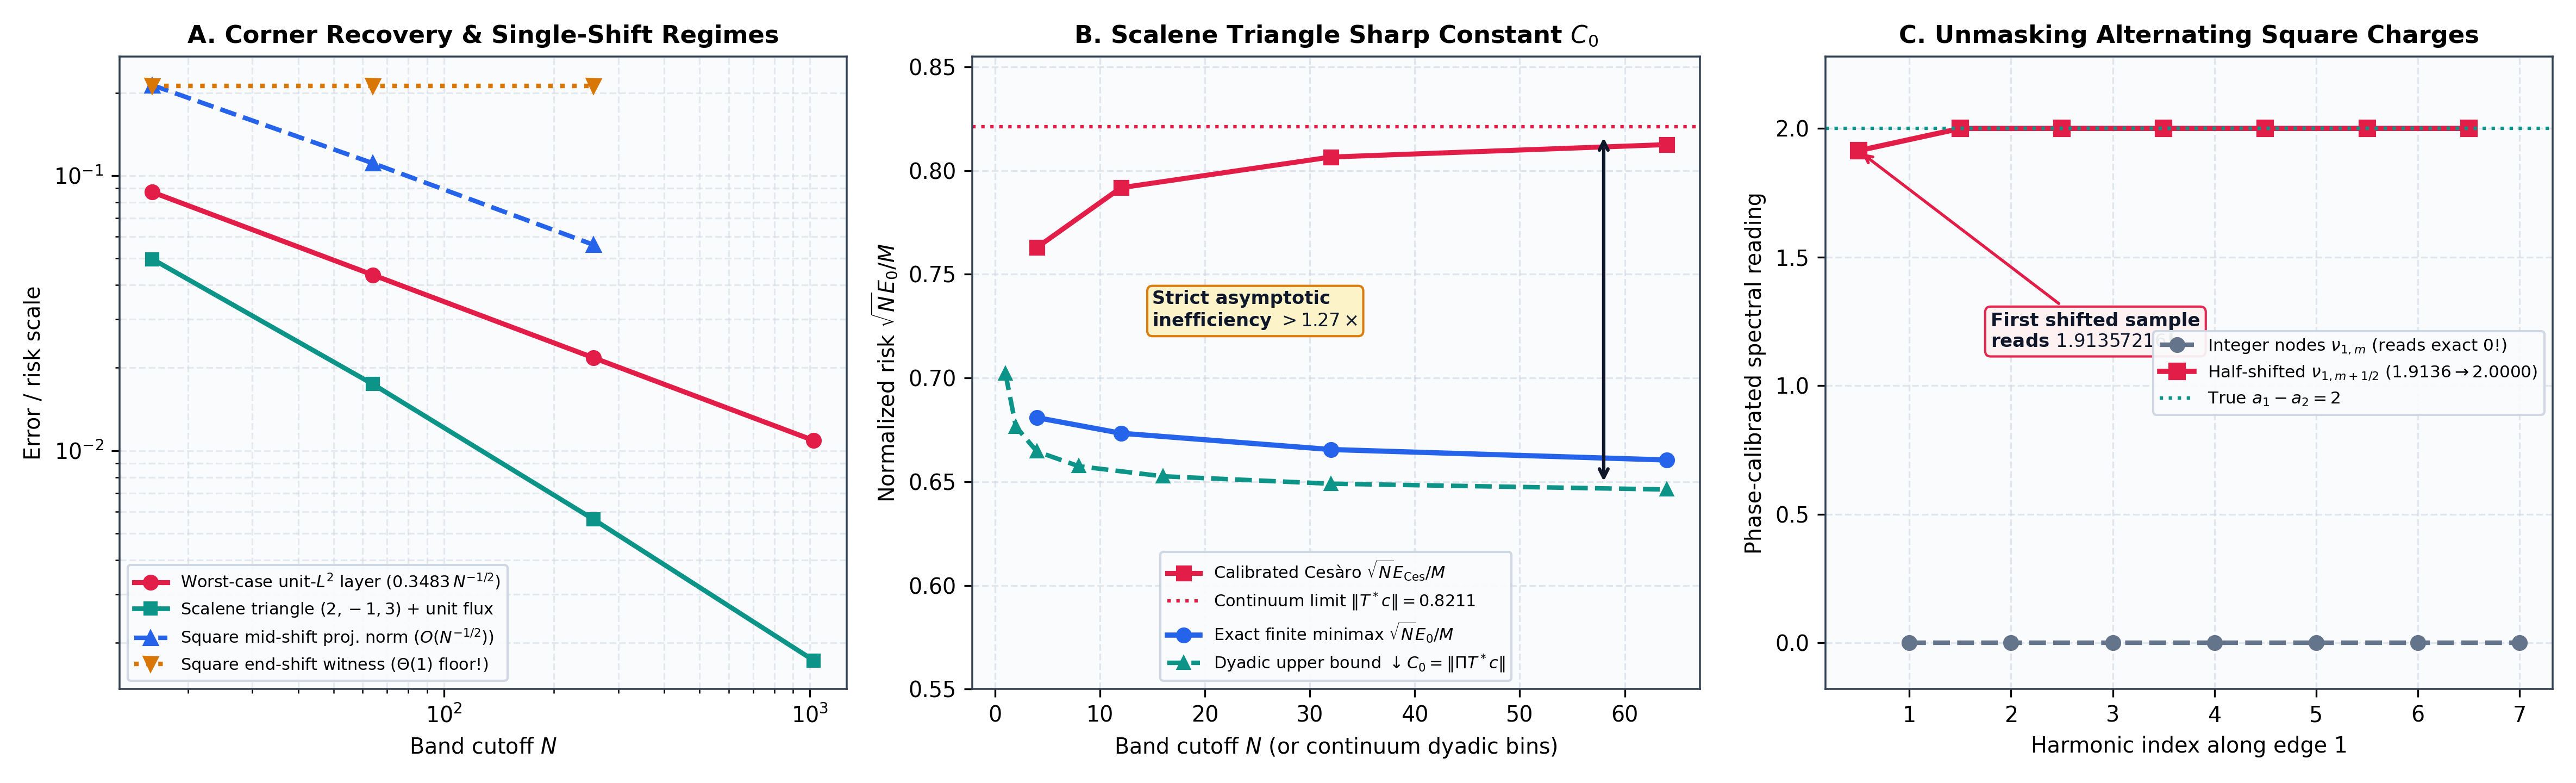
\includegraphics[width=\textwidth]{figs/p2_fig1_parity_and_minimax_odd.png}
\caption{\textbf{A.} Corner recovery on a scalene triangle, unit-$L^2$ boundary-layer witness $0.3483\,N^{-1/2}$ on a unit edge, and single-shifted-sample diagnostics on $[0,1]^2$ (mid-band own-edge Fourier projection norm $O(N^{-1/2})$ vs.\ end-of-band omitted-cardinal response $0.2122 = \Theta(1)$). \textbf{B.} Convergence of $\sqrt{N} E_0/M$ ($v_0 = \gamma_1$) on the scalene triangle $(0, 1.5+0.1i, 0.2+1.1i)$ toward $C_0 = \|\Pi T^*c^{(1)}\| \le 0.6463$, strictly below calibrated Ces\`aro ($\|T^*c^{(1)}\| = 0.8211$, $>27\%$ penalty on this vertex). \textbf{C.} Unmasking alternating square charges $(+1,-1,+1,-1)$: integer nodes read exact zero, while the half-shifted sequence $(m - 1 + \frac12)b_1$ ($m \ge 1$) starts at $2(1 - e^{-\pi}) = 1.91357216$ and converges to $2$.}
\label{fig:odd-parity}
\end{figure}

\section{Sharp Asymptotic Minimax Constant on Odd Polygons}\label{sec:odd}

Let $p = 2\kappa+1$ ($\kappa \ge 1$) be odd, and sample the first $N$ positive integer modes $\nu_{jm} = m b_j$ ($1 \le m \le N$, $1 \le j \le p$). At each vertex $v$, let $u$ range over the two unit vectors pointing into the two sides incident at $v$, and form the real Hilbert spaces
\[
  X = \bigoplus_{v,u} L^2(\R_+, \R), \qquad Y = L^2\bigl((0,1), \C^p\bigr) \quad\text{(equipped with }\operatorname{Re}\langle\cdot,\cdot\rangle\text{)}.
\]
Define the bounded tangent-ray Fourier--Laplace operator $T : X \to Y$ by
\begin{equation}\label{eq:T-op}
  (T f)_j(t) = \sum_{v \in \{\gamma_j,\gamma_{j+1}\}}\; \sum_{u \text{ at } v} \int_0^\infty e^{t b_j u x} f_{v,u}(x)\,dx, \qquad t \in (0,1).
\end{equation}
Own-side terms ($u = \pm d_j/|d_j|$) are bounded $L^2$ Fourier transforms by Plancherel; adjacent-side terms satisfy $\operatorname{Re}(b_j u) < 0$ and are bounded on $L^2(\R_+)$ by Schur's test on the Hilbert-type Laplace kernel $(x+y)^{-1}$ with weight $x^{-1/2}$. Let $P : Y \to Y$ be the real-orthogonal projection onto real constant vectors $\R^p \subset Y$, let $\Pi : X \to X$ be the orthogonal projection onto $\ker\bigl((I - P)T\bigr)$, and set $c^{(k)} = S^{-T} e_k \in \R^p$ ($1 \le k \le p$, viewed as a constant in $Y$).

\begin{theorem}[Sharp odd-polygon minimax constant and strict suboptimality of Ces\`aro]\label{thm:odd-constant}
On every genuine odd convex $p$-gon $D$ ($p = 2\kappa+1$) with $N$ integer nodes per edge, for every $M > 0$ and $1 \le k \le p$:
\begin{equation}\label{eq:odd-asymp}
  E_k(N) = \frac{M}{\sqrt{N}}\bigl(C_k + o(1)\bigr) \quad (N \to \infty), \qquad
  C_k = \|\Pi T^* c^{(k)}\|_X > 0.
\end{equation}
Moreover, calibrated uniform Ces\`aro averaging obeys $\lim_{N\to\infty} \sqrt{N} E_{k,\mathrm{Ces}}(N)/M = \|T^* c^{(k)}\|_X$, with strict asymptotic inefficiency
\begin{equation}\label{eq:cesaro-gap}
  \lim_{N\to\infty} \frac{E_{k,\mathrm{Ces}}(N)}{E_k(N)} = \frac{\|T^* c^{(k)}\|_X}{\|\Pi T^* c^{(k)}\|_X} > 1.
\end{equation}
\end{theorem}

\begin{proof}
\emph{Step 1: Scaling upper bound.} By Theorem~\ref{thm:finite-minimax}, $\sqrt{N} E_k(N)/M = \sup\{|a_k| : A a + R g = 0,\; \|g\|_{L^2(\partial D)} \le \sqrt{N}\}$. Take a maximizing sequence $(a^{(N)}, g^{(N)})$ with $\|g^{(N)}\|_2 \le \sqrt{N}$ and $A a^{(N)} + R g^{(N)} = 0$. Averaging the $N$ equations on each edge shows via Theorem~\ref{thm:endpoint-limit}(2) and invertibility of $S$ (Proposition~\ref{prop:parity}(1)) that $a^{(N)}$ is bounded. Splitting each edge at its midpoint and rescaling $f_{v,u}^{(N)}(x) = N^{-1} g^{(N)}(v + u x / N) \mathbf{1}_{[0, N|d|/2]}(x)$ satisfies $\|f^{(N)}\|_X \le 1$. Passing to a weakly convergent subsequence $f^{(N)} \rightharpoonup f \in X$ ($a^{(N)} \to a$) and testing against $N^{-1}\psi(m/N)$ for $\psi \in C_c^\infty(0,1)$ yields $T f + S a = 0$: on own half-edges, repeated summation by parts gives $O_b((1+x)^{-b})$ up to $N|d_j|/2$, while non-incident half-edges decay exponentially, so the Riemann-sum kernels converge strongly in $X$. Since $\|f\|_X \le 1$, $T f = -S a \in \R^p$ implies $(I - P) T f = 0$, i.e., $f \in \ker((I-P)T)$, and
\[
  a_k = \langle c^{(k)}, S a \rangle_Y = -\langle c^{(k)}, T f \rangle_Y = -\langle T^* c^{(k)}, f \rangle_X = -\langle \Pi T^* c^{(k)}, f \rangle_X,
\]
whence $|a_k| \le \|\Pi T^* c^{(k)}\|_X$, proving $\limsup_{N\to\infty} \sqrt{N} E_k(N)/M \le C_k$.

\emph{Step 2: Uniformly bounded cardinal interpolation and matching lower bound.} For $\nu = m b_j \in \Lambda_+$, define
\begin{equation}\label{eq:D-nu}
  D_\nu(s) = \frac{e^{\nu\gamma_j} L(s)}{(s - \nu) L'(\nu)} \left(\frac{s}{\nu}\right)^\kappa.
\end{equation}
Then $e^{-\nu'\gamma_{j'}} D_\nu(\nu') = \delta_{\nu,\nu'}$ on $\Lambda_+$ and $D_\nu(0) = 0$. By \eqref{eq:L-est}, along another ray $t b_\ell$ ($t > 0$), $|D_\nu(t b_\ell)| e^{-H(t b_\ell)} \le C \sqrt{m}(1+t)^{-1/2}/(m+t)$, whose $L^2(0,\infty)$ norm is $O(1)$ uniformly in $m$; on its own ray $t b_j$, replacing $m+t$ by $1 + |t - m|$ via the sine zero gives $L^2$ norm $O(1)$ as well. Applying the directional Laplace construction and Muckenhoupt $A_2$ Hilbert realification of \cite[Theorem~4.1]{Paper1} represents any complex multiple $\alpha D_\nu$ by a real density in $L^2(\partial D, \R)$ of norm $\le C_D |\alpha|$, uniformly in $\nu \in \Lambda_+$.

Now let $(a, f) \in \R^p \times X$ satisfy $\|f\|_X \le 1$ and $T f + S a = 0$, and fix $\varepsilon > 0$. Since $T[\lambda f(\lambda\,\cdot)](t) = (T f)(t/\lambda)$ and $\|\lambda f(\lambda\,\cdot)\|_X = \sqrt{\lambda}\,\|f\|_X \le \sqrt{1+\varepsilon}$, averaging $\lambda f(\lambda\,\cdot)$ against a smooth probability density supported in $[1, 1+\varepsilon]$ produces $f_\varepsilon \in X$ satisfying $T f_\varepsilon + S a = 0$ on $(0,1)$, $\|f_\varepsilon\|_X \le \sqrt{1+\varepsilon}$, and $f_\varepsilon^{(r)}(x) = o(x^{-1/2 - r})$ ($r = 0, 1, 2$) as $x \to \infty$. Rescaling $(a_\varepsilon, \widetilde f_\varepsilon) = (1+\varepsilon)^{-1/2}(a, f_\varepsilon)$ gives $\|\widetilde f_\varepsilon\|_X \le 1$. Transplanting $N \widetilde f_\varepsilon(N x)$ onto each incident side with a smooth cutoff vanishing before the midpoint has $L^2(\partial D)$ norm $\le (1 + o(1))\sqrt{N}$, and two integrations by parts on omitted oscillatory tails show that the $\ell^1$ sum of normalized sample discrepancies across $1 \le m \le N$ is $o(\sqrt{N})$. Correcting every sample error via linear combinations of \eqref{eq:D-nu} costs $o(\sqrt{N})$ in $L^2(\partial D)$, giving $\liminf_{N\to\infty}\sqrt{N}E_k(N)/M \ge (1+\varepsilon)^{-1/2}|a_k|$; sending $\varepsilon \downarrow 0$ and optimizing over $(a, f)$ proves $\liminf_{N\to\infty}\sqrt{N}E_k(N)/M \ge C_k$.

\emph{Step 3: Positivity $C_k > 0$ and strict Ces\`aro suboptimality.} To see $C_k > 0$, extend any bounded data $(y_{jm})_{m\le N}$ to $N < m \le 2N$ on each ray so that $\sum_{m=1}^{2N} y_{jm} e^{\nu_{jm}\gamma_j} / (\nu_{jm}^{\kappa+1} L'(\nu_{jm})) = 0$ (feasible with $|y_{jm}| = O(1)$ since $|\nu_{jm}^{\kappa+1} L'(\nu_{jm})|^{-1} e^{H(\nu_{jm})} \asymp m^{-1/2}$). Using $\frac{1}{s-\nu} + \frac{1}{\nu} = \frac{s}{\nu(s-\nu)}$, this cancellation raises the numerator power in $\sum_{m\le 2N} y_{jm} D_{\nu_{jm}}(s)$ to $s^{\kappa+1}$ for $|s| \le 4N$: on any dyadic shell $t \asymp J \le 4N$ the squared same-ray sum is $O(J)$ by integer-sinc orthogonality (and cross-ray sums have $L^2$ norm $O(\sqrt N)$), while for $t > 4N$ the unsubtracted representation is $O(N^{3/2} t^{-3/2})$, whose $L^2(4N,\infty)$ norm is $O(\sqrt N)$. Thus the realified $L^2(\partial D)$ density has norm $O_D(\sqrt{N})$. Applying this to unit vertex-charge data produces $(e_k, g^{(N)})$ with $\|g^{(N)}\|_2 \le C_D' \sqrt{N}$, whence $C_k \ge 1/C_D' > 0$.

Finally, calibrated Ces\`aro kernels rescale in $X$ to $T^* c^{(k)}$ by dominated convergence with majorant $C/(1+x)$. As $t \downarrow 0$, the own-side sinc kernel stays bounded under $T$, whereas the adjacent-side $1/x$ tail produces a logarithmic singularity $(T T^* c^{(k)})_j(t) = (L_j + L_{j+1})\log(1/t) + O(1)$ with $L_j = \sin\omega_j(c_{j-1}^{(k)}/|b_{j-1}| + c_j^{(k)}/|b_j|)$. If $(I - P) T T^* c^{(k)} = 0$, every logarithmic coefficient $L_j + L_{j+1}$ vanishes; invertibility of $S$ for odd $p$ forces $L_j = 0$ for all $j$, which in turn forces $c^{(k)} = 0$, a contradiction. Thus $T^* c^{(k)} \notin \ker((I-P)T)$, so $\|\Pi T^* c^{(k)}\|_X < \|T^* c^{(k)}\|_X$, proving \eqref{eq:cesaro-gap}.
\end{proof}

\begin{remark}[Convergent dyadic upper bounds]
Partitioning $(0,1)$ into $2^\ell$ equal subintervals and applying minimum-norm duality (via independent band rows or the pseudoinverse $G_\ell^\dagger$; indeed, wedge Poisson uniqueness and polynomial density on two-segment vertex trees imply full row rank) to the band-integrated rows of \eqref{eq:T-op}---whose Gram inner products evaluate in closed form via $(-tz - t'w)\Log(-tz - t'w)/(zw)$---yields a monotonically decreasing sequence converging to $C_k$ as $\ell \to \infty$ by nested weak compactness in $X$ (Figure~\ref{fig:odd-parity}B).
\end{remark}

\section{Even Polygons: Angle-Dependent Exponents and the Half-Step Myth}\label{sec:even}

Let $p = 2\kappa$ ($\kappa \ge 2$) be even. We augment the $p N$ integer nodes $\{\nu_{jm} : 1 \le j \le p,\; 1 \le m \le N\}$ with shifted nodes on edge $1$.

\begin{theorem}[Angle-dependent minimax order under a shifted edge band]\label{thm:even-exponent}
Let $D$ be a genuine even convex $p$-gon ($p = 2\kappa$) with interior angle $\omega_k \in (0,\pi)$ at vertex $\gamma_k$ ($1 \le k \le p$), and set $\beta_k = 2 - \omega_k/\pi \in (1, 2)$. Given the $p N$ integer samples together with $N$ shifted samples $\{(m - 1 + \theta) b_1 : 1 \le m \le N\}$ on edge $1$ ($0 < \theta < 1$), there exist constants $0 < c_D \le C_D < \infty$ such that for all sufficiently large $N$ and all $M \ge 0$ (uniformly in $0 < \theta < 1$ in exact arithmetic),
\begin{equation}\label{eq:even-rate}
  c_D M N^{-\beta_k / 2} = c_D M N^{-(1 - \omega_k/(2\pi))}
  \;\le\; E_k(N, \theta) \;\le\;
  C_D M N^{-(1 - \omega_k/(2\pi))}.
\end{equation}
\end{theorem}

\begin{proof}
Assume $M > 0$. By Theorem~\ref{thm:finite-minimax} and duality, $E_k(N,\theta)/M$ equals the minimum of $\|u\|_{L^2(\partial D)}$ over real combinations $u = \operatorname{Re} f$ of the $(p+1)N$ complex exponential rows satisfying $u(\gamma_\ell) = \delta_{k\ell}$ ($1 \le \ell \le p$). By Varga's arclength Christoffel theorem on piecewise smooth curves \cite[Theorem~2.4, Corollary~3.7]{Varga2013} (multiplied by fixed Lagrange cardinal polynomials $Q_k(\gamma_\ell) = \delta_{k\ell}$), the minimum boundary $L^2(\partial D)$ norm of an algebraic polynomial $P$ of degree $\le n$ satisfying $P(\gamma_\ell) = \delta_{k\ell}$ is $\asymp_D n^{-\beta_k/2}$. We establish two-sided exponential-polynomial comparisons at degree $n \asymp N$.

\emph{Upper bound}: Translate $D$ so $0 \in D$, set $b_* = \min_j |b_j|$, and form $F(s) = L(s) U(s)$ where $U(s) = \prod_{m=1}^J \bigl(s - (m-1+\theta)b_1\bigr)$ with $J = \lfloor \eta_0 N \rfloor > h + 1$ chosen small enough that $|(J-1+\theta)b_1| \le b_* N / 8$. Residue expansion on expanding circles gives $e^{tw} = \sum_{F(\lambda)=0} \frac{F(t)e^{\lambda w}}{(t-\lambda)F'(\lambda)}$ for $w \in \bar D$. Truncating to our measured rows omits only nodes $|\lambda| \ge b_* N$, where $|U(t)/U(\lambda)| \le (q_0 b_* N / |\lambda|)^J$ ($q_0 < 1$) for $|t| \le \eta N$. Using \eqref{eq:L-est} for $L'(\lambda)$ bounds the omitted tail uniformly on $\bar D$ by $C e^{C_D \eta N} N^{h+1} q_0^J = O(e^{-c N})$ for small fixed $\eta > 0$. Cauchy differentiation in $t$ at $t = 0$ approximates each monomial $w^\ell$ by measured rows within uniform error $O(e^{-c N} \ell! (\eta N)^{-\ell})$. First apply this approximation to the $p$ fixed Lagrange cardinal polynomials $Q_1,\dots,Q_p$ ($Q_r(\gamma_\ell) = \delta_{r\ell}$) to obtain real measured-row combinations $\widetilde u_1,\dots,\widetilde u_p$ whose vertex evaluation matrix satisfies $\widetilde u_r(\gamma_\ell) = \delta_{r\ell} + O(e^{-cN})$, hence is invertible for large $N$. Next approximate Varga's extremal polynomial $P$ of degree $n = \lfloor \eta r_0 N / 2 \rfloor$ ($B(0,r_0) \subset D$, $|p_\ell| \le C r_0^{-\ell}\|P\|_{L^2(\partial D)}$) by a real measured-row combination $u_P$, and subtract its $O(e^{-cN})$ vertex discrepancies using the inverted basis $\{\widetilde u_r\}_{r=1}^p$; this stays strictly inside the measured row space and achieves $u(\gamma_\ell) = \delta_{k\ell}$ with $\|u\|_{L^2(\partial D)} \le C_D N^{-\beta_k/2}$.

\emph{Lower bound}: Take any real measured-row combination $u = \operatorname{Re} f$ with $u(\gamma_\ell) = \delta_{k\ell}$, and set $f_0(z) = f(z) - i\operatorname{Im} f(0)$ so $\operatorname{Re} f_0 = u$ and $f_0(0) \in \R$. Pulling back to $\mathbb{D}$ via a centered Riemann map $\Phi$ with $|\Phi'| \in A_2(\mathbb{T})$ gives $\|f_0\|_{L^2(\partial D)} \le C_D \|u\|_{L^2(\partial D)}$, hence $|f_0(z)| \le C_D' \|u\|_2$ on a disk $|z| \le r_1$ inside $D$. Along any ray from $0$ to a large circle $|z| = R_1 > 2\max_{\bar D}|w|$, sampling $f_0$ at $L_0 = \lceil C_1 N \rceil$ equispaced radial steps produces a sum of $q \le (p+1)N + 1$ geometric progressions (including frequency $0$ from $-i\operatorname{Im}f(0)$) of ratios $|r_j| \le B_D$ whose first $q$ samples lie inside $|z| \le r_1$ (for $C_1$ large). Bounding the rational generating function $\sum_{m\ge 0} f_{0,m} \zeta^m = \text{Num}(\zeta)/\prod_{j=1}^q(1 - r_j\zeta)$ on $|\zeta| = (2\max\{1,B_D\})^{-1}$ bounds $|f_0|$ on $|z| = R_1$ by $e^{C_2 N}\|u\|_2$ independently of coefficient ill-conditioning! Truncating the Taylor series of $f_0$ at degree $n = \lceil C_3 N \rceil$ then leaves uniform error $O(e^{-N}\|u\|_2)$ on $\bar D$; applying Varga's polynomial lower bound at $\gamma_k$ yields $1 = u(\gamma_k) \le C N^{\beta_k/2}\|u\|_2 + O(e^{-N}\|u\|_2)$, proving $E_k(N,\theta)/M \ge c_D N^{-\beta_k/2}$.
\end{proof}

\begin{openproblem}[Exact asymptotic prefactor on even polygons]\label{op:even-prefactor}
Because the upper and lower polynomial comparisons in Theorem~\ref{thm:even-exponent} operate at distinct constant multiples of $N$, whether $N^{1 - \omega_k/(2\pi)} E_k(N,\theta)/M$ converges to a limit as $N \to \infty$, and which shift $\theta \in (0,1)$ minimizes that asymptotic prefactor, remain open.
\end{openproblem}

\begin{proposition}[Placement regimes for a single shifted sample]\label{prop:single-shift}
On an even convex $p$-gon ($p = 2\kappa$) with $M > 0$ and $1 \le k \le p$, suppose the $p N$ integer samples are augmented by \emph{only one} shifted sample at $\xi_N = (m_N + \theta) b_1$ ($0 < \theta < 1$).
\begin{enumerate}
  \item \emph{Fixed frequency ($m_N = m_0$ fixed)}: $\inf_{N \ge 1} E_k(N) > 0$ (inconsistent).
  \item \emph{Top of band ($m_N = N - 1$)}: $\inf_{N \ge 1} E_k(N) > 0$ (inconsistent).
  \item \emph{Proportional band interior ($m_N / N \to t_0 \in (0,1)$)}: $E_k(N) \asymp_{D,t_0,\theta} M N^{-1/2}$.
\end{enumerate}
(More generally, any interior placement with $\min\{m_N, N - m_N\} \to \infty$ restores consistency $E_k(N) \to 0$ via a centered projection of width $\min\{m_N, N - m_N\}$.)
\end{proposition}

\begin{proof}
(1) Choose $q \in \C \setminus \{0\}$ with $q C_{\gamma_1} \in \R$; then $F(s) = q s^{\kappa-1}(s - \xi) L(s)$ vanishes on $\Lambda_+ \cup \{\xi\}$ and by \cite[Theorem~4.1]{Paper1} represents a real measure with nonzero alternating corner masses $\pm q C_{\gamma_1}$ and $L^2$ residual density, creating an $N$-independent error floor. (2) Take the integer-invisible measure $\mu_0$ ($q s^\kappa L(s)$) with unit alternating atoms and cancel its nonzero response at $(N-1+\theta)b_1$ using the single omitted integer cardinal $D_{(N+1)b_1}$ (power $\kappa$ in \eqref{eq:D-nu}), which has bounded $L^2$ norm and response $\asymp 1$ at $(N-1+\theta)b_1$. (3) Subtracting $\sum_{|\ell|\le L_0} d_\ell h_{m_N+\ell}$ with $d_\ell = \frac{e^{2\pi i\theta}-1}{2\pi i(\theta-\ell)}$ ($L_0 \asymp N$) from the shifted row leaves own-edge norm $O(N^{-1/2})$, exponential damping on adjacent sides (pairing $\pm\ell$), and opposite limiting endpoint residuals $\pm\frac12(1 - e^{2\pi i\theta}) \ne 0$, giving $O(M/\sqrt N)$. Conversely, cancelling $\mu_0$'s shifted response with $N$ phase-aligned omitted cardinals $N < \ell \le 2N$ (each having modulus $\asymp N^{-1}$ at $(m_N+\theta)b_1$, while the $L^2(\partial D)$ norm of their sum is $O(\sqrt N)$ by same-ray integer-sinc orthogonality) gives $\Omega(M/\sqrt N)$.
\end{proof}

\begin{figure}[ht]
\centering
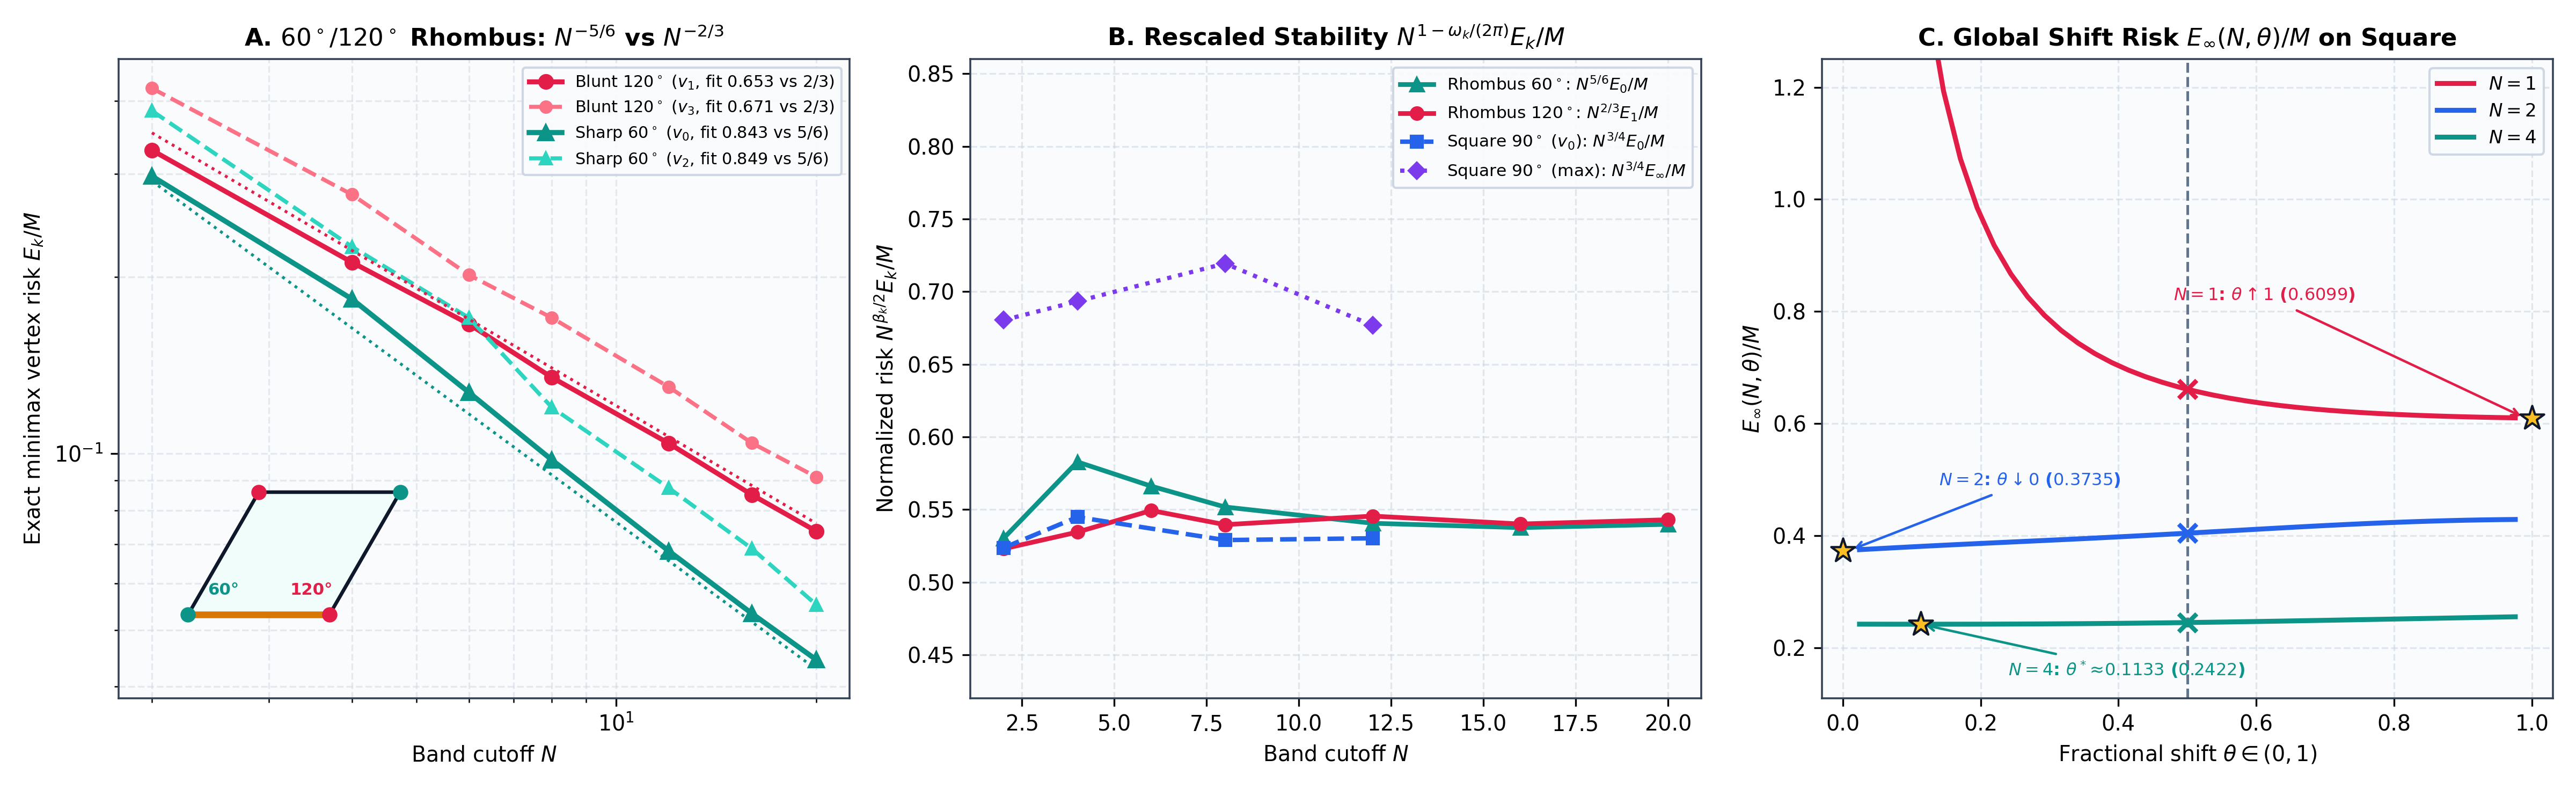
\includegraphics[width=\textwidth]{figs/p2_fig2_rhombus_and_shift_certificate.png}
\caption{\textbf{A.} Exact minimax vertex risks on the $60^\circ/120^\circ$ unit rhombus ($v_0=0, v_1=1, v_2=1+e^{i\pi/3}, v_3=e^{i\pi/3}$, half-shifted base edge; all 28 finite-band risks agree to all 45 saved significant digits between 100- and 132-digit runs): sharp $60^\circ$ corners follow $N^{-5/6}$ (fitted $0.843, 0.849$) while blunt $120^\circ$ corners follow $N^{-2/3}$ (fitted $0.653, 0.671$). \textbf{B.} Stability of $N^{1-\omega_k/(2\pi)} E_k/M$ across the rhombus ($60^\circ, 120^\circ$) and unit square ($90^\circ$, $N^{3/4}E_k/M$). \textbf{C.} Global shift curves $E_\infty(N,\theta)/M$ on $[0,1]^2$ for $N=1,2,4$: outward-rounded interval certificates prove $\theta = 1/2$ ($\times$) is never optimal; stars ($\star$) mark the certified interior optimum ($N=4$) and unattained endpoint limits ($N=1,2$).}
\label{fig:rhombus-shift}
\end{figure}

\begin{theorem}[Interval-certified suboptimality of the half-step on the unit square]\label{thm:square-shift}
On the unit square $[0,1]^2$ ($M = 1$), the global infimum of $E_\infty(N, \theta)$ over $\theta \in (0, 1)$ strictly beats the half-step $\theta = \frac12$ at each band $N \in \{1, 2, 4\}$:
\begin{center}
\footnotesize
\begin{tabular}{rlll}
\toprule
$N$ & Global optimizer / limit in $(0,1)$ & Certified $\inf_\theta E_\infty(N,\theta)$ & Half-step $E_\infty(N, 1/2)$ \\
\midrule
$1$ & Limit $\theta \uparrow 1$ (unattained) & $[0.60987939561604939,\, \dots 40]$ & $0.6612539973234749\dots$ \\
$2$ & Limit $\theta \downarrow 0$ (unattained) & $[0.37347544568190208,\, \dots 09]$ & $0.4045541022567613\dots$ \\
$4$ & Unique $\theta^* \in [0.11329911665530738903,\, \dots 09]$ & $[0.24216109141774661,\, \dots 62]$ & $0.2451356264257993\dots$ \\
\bottomrule
\end{tabular}
\end{center}
\end{theorem}

\begin{proof}
Writing $J(\theta) = \bigl(\begin{smallmatrix} G(\theta) & A(\theta) \\ A(\theta)^T & 0 \end{smallmatrix}\bigr)$, $K_{kk}(\theta)$ equals minus the $k$-th atom diagonal cofactor divided by $\det J(\theta)$. Divided-difference row stabilization replaces colliding rows as $\theta \uparrow 1$ (or at collisions with sampled positive integer nodes $m b_1$) by the full complex spectral derivative $b_1 B_\mu'(m b_1)$, whereas as $\theta \downarrow 0$ the first shifted node $(0+\theta)b_1 \to 0$ approaches the unsampled origin, contributing the real total mass $B_\mu(0)$ and directional moment $\operatorname{Im}(b_1 B_\mu'(0))$ (at $N=1$, $\theta\downarrow 0$ leaves $A$ rank-deficient and $E_\infty$ diverges). Using 230-decimal outward-rounded interval arithmetic (\texttt{mp.iv}, derivative-error bound $< 10^{-36}$, risks rounded outward to 17 decimals), our subdivision certificate establishes the monotone derivative signs of the active vertex branch and its strict dominance over the complementary vertex branch near the minimizer, proving the stated brackets (Figure~\ref{fig:rhombus-shift}C).
\end{proof}

\section{Smooth-Background Super-Resolution and the Chebyshev Barrier}\label{sec:superres}

When the diffuse flux $g$ is edgewise smooth, ordinary Ces\`aro means generically stall at rate $O((\log N)/N)$ (or $O(N^{-1})$ when the leading term cancels) due to $O(m^{-1})$ endpoint terms from integration by parts. Fix an \emph{identifying edge-group design}: the $p$ integer edge groups ($x_m = m$) for odd $p$, and those $p$ integer groups plus one shifted group on edge~$1$ ($x_m = m - 1 + \theta$, fixed $\theta \in (0,1)$) for even $p$, writing $t_m = x_m / N$.

\begin{theorem}[Inverse-power-cancelling windows and Chebyshev lower bound]\label{thm:superres}
Fix the identifying edge-group design above.
\begin{enumerate}
  \item \emph{Smooth-bump projection windows}: Fix $r \in \Z_{\ge 1}$ and nonnegative nonzero $\chi \in C_c^\infty((a,b))$ ($0 < a < b < 1$). For all sufficiently large $N$, $H_{\ell j} = \sum_{m=1}^N \chi(t_m) t_m^{-\ell-j}$ ($0 \le \ell, j \le r$) is invertible, and $w_m = \chi(t_m)\sum_{j=0}^r (H^{-1} e_0)_j t_m^{-j}$ satisfies $\sum_{m=1}^N w_m = 1$, $\sum_{m=1}^N w_m x_m^{-\ell} = 0$ ($1 \le \ell \le r$), $\|w\|_1 = O_r(1)$, and $\|w\|_2 = O_r(N^{-1/2})$. The resulting vertex-calibrated estimator achieves
  \begin{equation}\label{eq:smooth-rates}
    \sup_{a,\,\max_j \|g|_{\Gamma_j}\|_{C^r} \le M} \|\widehat a - a\|_\infty = O_{D,r}\bigl(M N^{-r-1}\bigr), \quad
    \sup_{a,\,\max_j \|g|_{\Gamma_j}\|_{H^r} \le M} \|\widehat a - a\|_\infty = O_{D,r}\bigl(M N^{-r-1/2}\bigr),
  \end{equation}
  and both exponents are sharp for this window estimator.
  \item \emph{Analytic exponential super-resolution}: On equispaced positive nodes $x_i = x_0 + i d > 0$ ($0 \le i \le r$, $x_i \in [a N, b N]$, $d \asymp N/r$), the explicit extrapolation weights
  \begin{equation}\label{eq:extrap-weights}
    w_i = \frac{(-1)^{r-i} x_i^r}{d^r\, i!\,(r - i)!}, \qquad 0 \le i \le r,
  \end{equation}
  satisfy $\sum_{i=0}^r w_i = 1$ and $\sum_{i=0}^r w_i x_i^{-\ell} = 0$ ($1 \le \ell \le r$). If each $g|_{\Gamma_j}$ extends holomorphically to a fixed neighborhood $U_j \supset \Gamma_j$ of the closed edge with $\sup_{U_j}|g_j| \le M$, choosing $r = \lfloor \varepsilon N \rfloor$ ($\varepsilon > 0$ small) yields $O(M e^{-c N})$ exponential vertex recovery.
  \item \emph{Universal Chebyshev amplification bound}: Any weights $(w_m)$ supported on at most $N$ sample indices in $[a N, b N]$ ($0 < a < b$) satisfying $\sum w_m = 1$ and $\sum w_m x_m^{-\ell} = 0$ ($1 \le \ell \le r$) obey
  \begin{equation}\label{eq:chebyshev}
    \|w\|_1 \ge \left|T_r\!\left(\frac{a+b}{b-a}\right)\right|, \qquad
    \|w\|_2 \ge \frac{1}{\sqrt{N}}\left|T_r\!\left(\frac{a+b}{b-a}\right)\right|,
  \end{equation}
  where $T_r$ is the degree-$r$ Chebyshev polynomial of the first kind.
\end{enumerate}
\end{theorem}

\begin{proof}
(1) Since $H/N$ converges to a positive definite continuous Gram matrix on $[a,b]$, $H$ is invertible for large $N$ with $\|H^{-1}e_0\| = O_r(N^{-1})$, giving $\|w\|_1 = O_r(1)$, $\|w\|_2 = O_r(N^{-1/2})$, and $|\Delta^{b_0} w_m| = O_r(N^{-1-b_0})$. Under the identifying design, the weighted vertex-response matrix $V A$ converges to the invertible endpoint matrix of Proposition~\ref{prop:parity}, so $\|(V A)^\dagger\| = O_{D,\theta}(1)$. Integrating $\int_{\Gamma_\ell} e^{x_m b_j(w-\gamma_j)} g(w)\,d\ell$ by parts $r$ times produces endpoint jets $g^{(\ell-1)}$ ($\ell \le r$) multiplied by $x_m^{-\ell}$---which sum to zero against $w_m$ at exposed endpoints and are $O(e^{-c_2 N})$ at damped endpoints---plus an integral against $g^{(r)}$ whose kernel has $L^1$ norm $O_r(N^{-r-1})$ and $L^2$ norm $O_r(N^{-r-1/2})$ via summation by parts; an incident bump of width $\varepsilon/N$ proves sharpness for this window estimator.

(2) Multiplying $w_i x_i^{-\ell}$ by $d^r r!$ yields $\sum_{i=0}^r (-1)^{r-i} \binom{r}{i} (x_0 + i d)^{r-\ell}$, the $r$-th forward difference of a degree-$(r-\ell)$ polynomial, equal to $r! d^r$ for $\ell = 0$ and $0$ for $1 \le \ell \le r$ (verified over $\mathbb{Q}$ in Lean~4 module \texttt{SuperResolutionWindow}, extending to $\R$ by clearing denominators). Here $\|w\|_1 \le C_0^r$. Uniform Cauchy estimates $|g^{(\ell)}| \le M C_1^\ell \ell!$ on $\Gamma_j \subset U_j$ bound both the $r$-th integration-by-parts remainder and the damped non-exposed endpoint jets by $O\bigl(M (C_0 C_1 r/(aN))^r + M C_0^r e^{-c_2 N}\bigr) = O(M e^{-cN})$ for $r = \lfloor \varepsilon N \rfloor$ with $\varepsilon < \min\{a/(e C_0 C_1), c_2/(2\log C_0)\}$.

(3) Setting $u_\pm = \frac12(a^{-1} \pm b^{-1})$, define $P(u) = T_r\bigl((u - u_+)/u_-\bigr) / T_r(-u_+/u_-)$. Then $\deg P = r$, $P(0) = 1$, and $|P(u)| \le |T_r(\frac{a+b}{b-a})|^{-1}$ for all $u = N/x_m \in [b^{-1}, a^{-1}]$. Moment cancellation gives $1 = P(0) = \sum_m w_m P(N/x_m) \le \|w\|_1 \max_m |P(N/x_m)|$, and Cauchy--Schwarz over $\le N$ indices gives $\|w\|_2 \ge N^{-1/2}\|w\|_1$.
\end{proof}

\begin{figure}[ht]
\centering
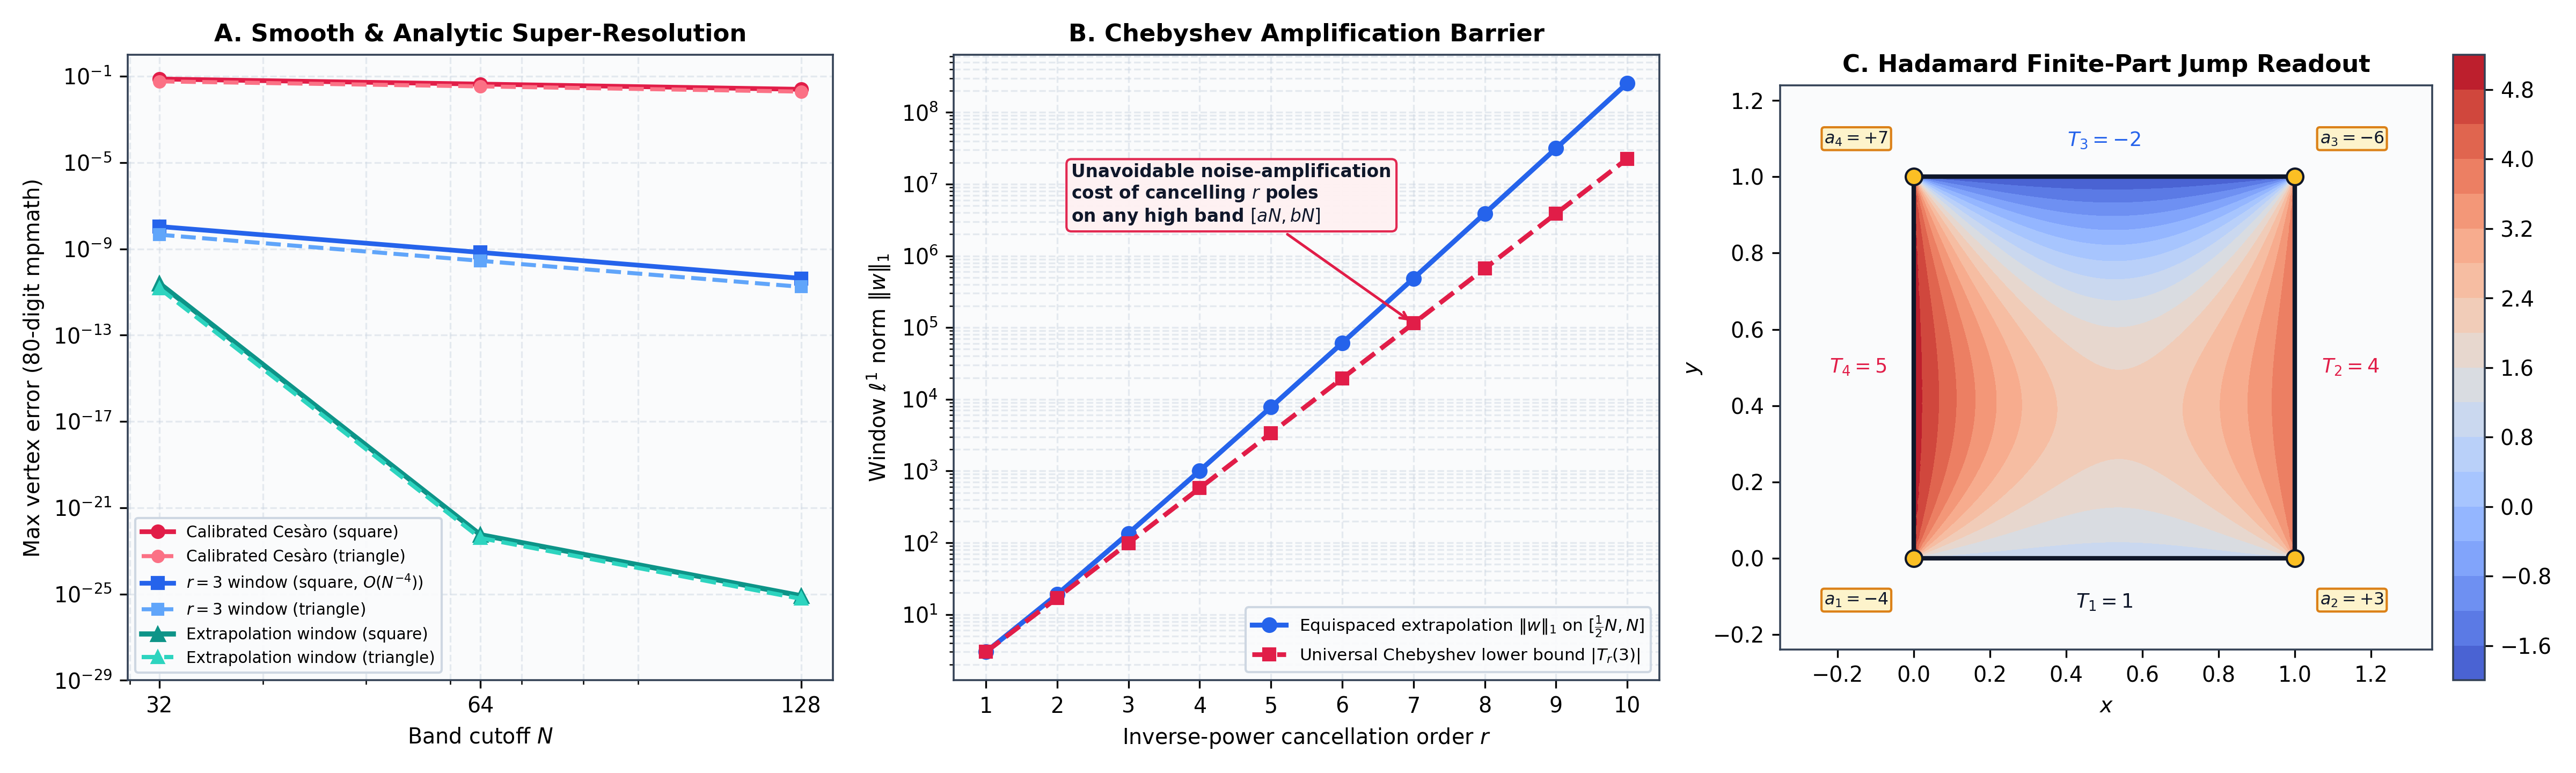
\includegraphics[width=\textwidth]{figs/p2_fig3_superresolution_and_heat_plate.png}
\caption{\textbf{A.} Smooth-background vertex recovery ($g|_{\Gamma_j}(t) = (1+j/4)e^{(j+1)t/5}$) on the scalene triangle and unit square: order-$8$ extrapolation windows improve accuracy at $N=128$ from $1.93\times 10^{-2}$ to $6.05\times 10^{-26}$ on the triangle and from $2.47\times 10^{-2}$ to $8.30\times 10^{-26}$ on the square ($\approx 23.5$ orders of magnitude). \textbf{B.} Equispaced extrapolation norm $\|w\|_1$ on $[\frac12 N, N]$ vs.\ the universal Chebyshev lower bound $|T_r(3)|$. \textbf{C.} Steady temperature field $q(x,y)$ on $[0,1]^2$ with discontinuous wall temperatures $(1,4,-2,5)$ and Hadamard finite-part jump readout ($7.1\times 10^{-14}$ agreement).}
\label{fig:superres-plate}
\end{figure}

\section{Discontinuous Wall Temperatures and Hadamard Finite-Part Flux}\label{sec:plates}

Finally, let $q$ be the bounded harmonic solution of $\Delta q = 0$ in $D$ with piecewise constant wall temperatures $q|_{\Gamma_j} = T_j \in \R$, jumping by $a_j = T_j - T_{j-1}$ at vertex $\gamma_j$ ($\sum_{j=1}^p a_j = 0$). Then the tangential derivative is purely atomic, $q_t = \sum_{j=1}^p a_j \delta_{\gamma_j}$, while near vertex $\gamma_j$ (in polar coordinates $(r,\varphi)$ with $\varphi = 0$ on outgoing $\Gamma_j$ and $\varphi = \omega_j$ on incoming $\Gamma_{j-1}$), sector straightening $z^{\pi/\omega_j}$ and odd reflection yield
\begin{equation}\label{eq:corner-sing}
  q(r,\varphi) = T_j - \frac{a_j}{\omega_j}\varphi + O\bigl(r^{\pi/\omega_j}\bigr), \qquad
  q_{n,\mathrm{out}}(r) = \frac{a_j}{\omega_j r} + O\bigl(r^{\pi/\omega_j - 1}\bigr), \quad
  q_{n,\mathrm{in}}(r) = -\frac{a_j}{\omega_j r} + O\bigl(r^{\pi/\omega_j - 1}\bigr).
\end{equation}
Thus at every vertex with $a_j \ne 0$, $q_n$ fails both $L^1(\partial D)$ and weak-$L^2(\partial D)$ on each incident side! Pairing incoming and outgoing sides at equal physical radii $\varepsilon \downarrow 0$ defines the two-sided Hadamard finite part $\langle \fp q_n, h \rangle := \lim_{\varepsilon\downarrow 0} \int_{\partial D \setminus \bigcup_j B(\gamma_j,\varepsilon)} q_n h\,d\ell$.

\begin{theorem}[Hadamard finite-part heat-flux identity]\label{thm:plate}
For every entire holomorphic test function $h \in H(\C)$ (in particular $h(w) = e^{sw}$),
\begin{equation}\label{eq:fp-identity}
  \langle \fp q_n, h \rangle = i \sum_{j=1}^p a_j h(\gamma_j), \qquad
  B_{\fp q_n}(s) = i \sum_{j=1}^p a_j e^{s\gamma_j}.
\end{equation}
Consequently, normalized Ces\`aro averages of $B_{\fp q_n}$ at $\nu_{j,m+\theta}$ converge to $i(a_j + e^{2\pi i\theta}a_{j+1})$: odd polygonal plates reveal all temperature jumps from integer modes alone, whereas on even plates the alternating jump mode $a_j = (-1)^j c$ ($\sum a_j = 0$) vanishes in the limiting integer endpoint-sum map (and identically at all integer nodes on parallelograms/squares, though not necessarily at individual finite nodes on general even polygons; cf.\ \cite[Remark~4.2]{Paper1}), and is universally recovered by adding one shifted edge.
\end{theorem}

\begin{proof}
Apply Green's second identity to $q$ and $h$ on $D_\varepsilon = D \setminus \bigcup_{j=1}^p B(\gamma_j,\varepsilon)$. On the small circular arcs $\partial B(\gamma_j,\varepsilon) \cap D$, $\int q\,\partial_n h\,d\ell = O(\varepsilon) \to 0$ since $q$ is bounded, while $\partial_r(T_j - a_j\varphi/\omega_j) = 0$ and $\partial_r O(r^{\pi/\omega_j}) = O(\varepsilon^{\pi/\omega_j - 1})$ with $\pi/\omega_j > 1$ give $\int h\,\partial_n q\,d\ell = O(\varepsilon^{\pi/\omega_j}) \to 0$. Because the opposite $\pm a_j/(\omega_j r)$ logarithmic divergences cancel at equal cutoff $\varepsilon$, passing to $\varepsilon \downarrow 0$ gives $\langle \fp q_n, h \rangle = \int_{\partial D} q\,\partial_n h\,d\ell$ for any smooth harmonic $h$; when $h$ is holomorphic, the Cauchy--Riemann relation $\partial_n h = -i\partial_t h$ yields $\int_{\partial D} q\,\partial_n h\,d\ell = -i \sum_{j=1}^p T_j \bigl(h(\gamma_{j+1}) - h(\gamma_j)\bigr) = i \sum_{j=1}^p (T_j - T_{j-1}) h(\gamma_j)$, proving \eqref{eq:fp-identity}. Independent Schwarz--Christoffel pullbacks of the principal-value Poisson flux on $\mathbb{D}$ confirm \eqref{eq:fp-identity} to $6.5\times 10^{-14}$ on the equilateral triangle and $7.1\times 10^{-14}$ on the square (Figure~\ref{fig:superres-plate}C).
\end{proof}

\subsection*{Lean~4 formal verification summary}
Three standalone Lean~4.36.0 modules accompany the algebraic core of this paper with zero \texttt{sorry} declarations and standard foundational axioms only (\texttt{propext}, \texttt{Classical.choice}, \texttt{Quot.sound}): \texttt{PolygonParity.lean} (cyclic parity invertibility and single-shift inversion in Proposition~\ref{prop:parity}), \texttt{FiniteMinimax.lean} (finite-dimensional saddle-point algebra and arbitrary nonlinear estimator lower bounds under the matrix/witness hypotheses of Theorem~\ref{thm:finite-minimax}), and \texttt{SuperResolutionWindow.lean} (rational finite-difference normalization and inverse-power annihilation in Theorem~\ref{thm:superres}(2)). Polygon Gram positivity, $L^2$ observation models, and analytic asymptotics are supplied by Sections~\ref{sec:minimax}--\ref{sec:superres} above.

\begin{thebibliography}{99}

\bibitem{Ashton2012}
A.~C.~L. Ashton, \emph{The spectral Dirichlet--Neumann map for Laplace's equation in a convex polygon}, SIAM J. Math. Anal. \textbf{45} (2013), no.~6, 3575--3591.

\bibitem{AshtonFokas2013}
A.~C.~L. Ashton and A.~S. Fokas, \emph{Elliptic boundary value problems in convex polygons with low regularity boundary data via the unified method}, preprint, arXiv:1301.1490 (2013).

\bibitem{DFPW2019}
R.~DeVore, S.~Foucart, G.~Petrova, and P.~Wojtaszczyk, \emph{Computing a quantity of interest from observational data}, Constr. Approx. \textbf{49} (2019), 461--508.

\bibitem{Donoho1994}
D.~L. Donoho, \emph{Statistical estimation and optimal recovery}, Ann. Statist. \textbf{22} (1994), no.~1, 238--270.

\bibitem{FFX2004}
S.~R. Fulton, A.~S. Fokas, and C.~A. Xenophontos, \emph{An analytical method for linear elliptic PDEs and its numerical implementation}, J. Comput. Appl. Math. \textbf{167} (2004), 465--483.

\bibitem{Leontev1974Polygon}
A.~F. Leont'ev, \emph{On the representation of an analytic function as a sum of periodic functions}, Mat. Sb. \textbf{93(135)} (1974), no.~4, 512--528; English transl. in Math. USSR-Sb. \textbf{22} (1974), 517--534.

\bibitem{Leontev1976Book}
A.~F. Leont'ev, \emph{Ryady eksponent} [\emph{Series of Exponentials}], Nauka, Moscow, 1976 (in Russian).

\bibitem{Leontev1987TrMIAN}
A.~F. Leont'ev, \emph{Series and sequences of polynomials of exponentials}, Trudy Mat. Inst. Steklov. \textbf{176} (1987), 308--325; English transl. in Proc. Steklov Inst. Math. \textbf{176} (1988), 309--326.

\bibitem{MicchelliRivlin1977}
C.~A. Micchelli and T.~J. Rivlin, \emph{A survey of optimal recovery}, in Optimal Estimation in Approximation Theory, Plenum, New York, 1977, pp.~1--54.

\bibitem{Paper1}
Project ReMath, \emph{Invisible boundary loads on convex polygons: Leont'ev's exponential lattice, balayage anatomy, and Fokas's global relation}, companion paper, 2026.

\bibitem{Varga2013}
T.~Varga, \emph{Christoffel functions for doubling measures on quasismooth curves and arcs}, Acta Math. Hungar. \textbf{141} (2013), 161--184.

\end{thebibliography}

\end{document}
